\documentclass[conference]{IEEEtran}
\IEEEoverridecommandlockouts
% The preceding line is only needed to identify funding in the first footnote. If that is unneeded, please comment it out.
\usepackage{cite}
\usepackage{amsmath,amssymb,amsfonts}
\usepackage{algorithmic}
\usepackage{graphicx}
\usepackage{textcomp}
\usepackage{xcolor}
\usepackage{hyperref} % For hyperlinks in the PDF
\def\BibTeX{{\rm B\kern-.05em{\sc i\kern-.025em b}\kern-.08em
    T\kern-.1667em\lower.7ex\hbox{E}\kern-.125emX}}
\begin{document}

\title{Genetic Algorithms for Interactive Music Creation\\
    % This footnote is usually used for funding; we acknowledge course staff 
    % here instead. They granted us w/ knowledge, I suppose?
    \thanks{This project was done for AA222/CS361: Engineering Design Optimization.
        The code is available on GitHub at
        \href{https://github.com/garrickf/genalg-sequencer}{garrickf/genalg-sequencer}.
        Thanks to Prof. Mykel Kochenderfer and the rest of the teaching team for their
        feedback on the project and a great class!}
}

\author{\IEEEauthorblockN{Garrick Fernandez}
    \IEEEauthorblockA{\textit{Department of Computer Science} \\
        \textit{Stanford University}\\
        Stanford, CA\\
        garrick@cs.stanford.edu}
}

\maketitle

\begin{abstract}
    Genetic algorithms have been applied to a number of problems, including the
    composition and generation of music. More broadly, computers are a cornerstone
    of the music-making process, often utilized for the arrangement and synthesis
    of new sounds. In this paper, we apply genetic algorithms to the task of music
    creation, with an eye towards live feedback and interactive performance. Our
    main contributions are (1) a formalization of the application of genetic
    algorithms to sound synthesis and rhythmic sequencing, (2) an exploration of
    human input and methods for fitness approximation, and (3) the production and
    interpretation of generated music.
\end{abstract}

\begin{IEEEkeywords}
    genetic algorithms, evolutionary music, sound synthesis, fitness approximation
\end{IEEEkeywords}

\section{Introduction}
Computers have been applied to the generation and composition of music since
the 1950's, and as such, the field of computer music is vast. Genetic
algorithms have seen use in a number of problem domains. This project seeks to
apply genetic algorithms to the problem of music creation. In addition, we wish
to incorporate human feedback as a mechanism by which the genetic algorithm
proceeds. We first formalize the problem and describe the method and
implementation used to optimize it. We then present results on the music
generation and progression of our algorithm.

\section{Problem}
There are many creative aspects to music we may wish to augment with a genetic
algorithm. To formalize our problem, we consider a simplification of the music
generation task, taking inspiration from step sequencers.\footnotemark
\footnotetext{Of particular inspiration to the author were Pocket
    Operators, handheld drum synthesizers and sequencers designed by Teenage Engineering.}

A sequencer \cite{sequencers} records, stores, and plays back music; it is
operated or programmed by a musician. All sequencers must store some form of
note and performance information; they may produce sounds with one or more
voices, or unique timbres (think of the difference between a trumpet and a
tuba).

In lieu of exact timing, a step sequencer rounds note triggers to the nearest
whole beat. Usually a grid of 16 buttons is provided to allow toggling a note
to play on a certain beat. At each step, or beat, a note is either triggered,
or it is not. This 16-beat measure loops indefinitely.

The tradeoff in the precision and beat-accurate timing of step sequencers is
that timing variation due to expressive performance is non-existent. As such,
this style of sequencing lends itself well to drum machines and electronic
music.

With this perspective, we can model music as a collection of chosen voices
(``parts'') performing different notes at discretized timings. A single part in
our sequencer can be thought of as an individual design point which encodes
information about its voice and trigger time information. A musical collection
of parts is a collection of design points. The formal goal of our genetic
algorithm is to optimize these design points and produce better parts, with
``better'' being dependent on the user/listener's tastes.

An important aspect of our task is integrating the genetic algorithm into a
human-centered music production process. When creating music, one can imagine
starting a song with a single track, then introducing and layering more tracks
as time goes on. Some tracks may be better or worse than others, creating
selection pressure on the track. As such, we focus on methods which optimize
with respect to a population of chromosomes, and allow the user to pick those
individuals they like for inclusion in their pieces.

Another perspective on our task is that we seek to incorporate genetic
algorithms into the exploration process for sounds and patterns in a
synthesizer/sequencer. The human operator is not removed from this process;
rather, they close a loop between the genetic algorithm and the music,
providing feedback to the genetic algorithm and thereby manipulating the
outputted sound.

\section{Method}

Genetic algorithms fall under a larger class of optimization techniques,
population methods, which involve optimization using a collection of design
points. In particular, genetic algorithms borrow inspiration from biological
evolution \cite{genalg-textbook,textbook}. In order to apply genetic algorithms to our
task, we must specify how to encode our music as genetic material, as well as
the mechanisms with which it evolves over time.

\subsection{Chromosome Structure and Representation}

To represent points associated with individuals in the design space, we used
real-valued chromosomes ($n$-dimensional vectors in
$\mathbb{R}^n$) with some components constrained to be integers. Each
chromosome is interpreted as having three main portions:

\begin{enumerate}
    \item A single positive integer $k \in \{1, \dots K\}$, the ``instrument,'' encodes
          which voice is used, where $K$ is the total number of voices
          available to the
          sequencer.
    \item A $\mathbb{R}^{n_\text{emb}}$ chunk of the chromosome, the
          ``expression,'' encompasses all points in the design space for instrument
          $k$.
          Client code in an audio synthesis program can ingest these numbers and map them
          to properties of the instrument (such as the frequency, filter cutoff, reverb,
          attack, etc.). For us, $n_\text{emb} = 16$.
    \item An $\{0, 1\}^{n_\text{tim}}$ chunk of the chromosome, the "timing," encodes trigger
          time information (1 if the note should play on time-step $t \in \{1, \dots, n_\text{tim}\}$,
          0 otherwise). For us, $n_\text{tim} = 16$, corresponding to the typical grid
          of
          sixteen steps seen in step sequencers.
\end{enumerate}

It follows that the dimension of our chromosomes is
\begin{equation}
    1 + n_\text{emb} + n_\text{tim} = 33
\end{equation}

The inclusion of an expression component allows the genetic algorithm to
perform exploratory  sound synthesis in addition to sequencing notes. The
parameters and bounds of this exploration are set by client (instrument) code.
Because of this, a programmer or musician retains some control over the
expression of their instruments through the way they interpret incoming design
points. However, the genetic algorithm remains the process by which these
design points are evaluated and improved. This decoupling grants flexibility in
terms of being able to create new instruments, or a new suite of instruments,
which react to expression parameters in different ways.

\subsection{Evolutionary Dynamics}

All genetic algorithms require instructions for how to produce the initial
population of chromosomes, how to perform selection, how to perform crossover
of genetic material between two parents, and how to perform mutation of a
chromosome. We refer to these jointly as the evolutionary dynamics of the
genetic algorithm.

For each individual in the initial population, the instrument is drawn from a
categorical distribution assigning equal probability mass to each instrument
$k \in \{1, \dots, K\}$. The expression information is sampled from a uniform
distribution between 0 and 1 for each coordinate. Since trigger times can only
be 0 or 1, we sample from a Bernoulli distribution for each of the sixteen time
steps. The distribution is weighted more towards sounding a note
($p=0.75$), so that the algorithm starts off with denser rhythms,
although this can be tuned.

Selection determines which chromosomes will be parents for the next generation.
We considered two approaches for selection. The first method considered was
truncation selection, where we sample from the top-$k$
chromosomes in the population.

The second selection method we considered was roulette wheel selection, also
known as fitness proportionate selection. In this method, each parent is chosen
with a probability proportional to its performance relative to the rest of the
population. Compared to truncation selection, roulette wheel gives a small
chance of less fit individuals being selected, which can help maintain genetic
variability in future generations.

Our method for implementing roulette wheel selection involved computing the
maximum objective value $y_\text{max}$ among objective values
$y_1, \dots, y_{N_\text{pop}}$, where $N_\text{pop}$ is the population size.
Then, the selection likelihood for an individual with objective value
$y_i$ would be:
%
\begin{equation}
    \frac{y_\text{max} -
    y_i}{\sum_{j=1}^{N_\text{pop}} y_\text{max}
    - y_j}\label{roulette-sel}
\end{equation}

Since smaller objective values are more optimal (we use the convention of
minimization), the smaller $y_i$ is, the larger the difference
between it and $y_\text{max}$. Thus the smallest $y_i$
values are associated with the highest chances for selection. In this scheme,
the worst-performing individual will have zero probability mass assigned to it,
as the numerator in \eqref{roulette-sel} would be zero.

In both selection methods, the sampling process is repeated multiple times to
select two parents for each of the $N_\text{pop}$ offspring.

Crossover is the process by which two parents combine their genetic material to
form children. There are multiple approaches to crossover; for our application,
we use a modified version of uniform crossover that behaves differently for
each portion of the parent chromosomes. In this method, instrument and
expression information are selected from either parent with equal probability.
For timing information, however, a four-beat bar is selected from either parent
with equal probability. This choice was to attempt to preserve an element of
phrasing a listener may experience when hearing music—some beats are
perceptually grouped together into a unit with its own musical sense, and a
user may want to preserve or explore these traits more. We leave it to the
mutation operation to produce trigger timing variations at the more
fine-grained, beat-by-beat level.

Mutation allows new traits to appear in the population, driving the exploration
of the genetic algorithm. For our application, we mutate each component in the
chromosome (resample it) with some fixed probability. In our implementation,
the probabilities are specific to the the instrument, expression, and timing
regions of the chromosome, and they can be modified.

\subsection{Fitness Approximation Based on User Feedback}

Selection in a genetic algorithm happens with respect to a fitness function
over the individuals in a population. Our fitness function is dependent on the
user's tastes, which are not known prior to the start of the algorithm. One
idea is to collect observations of the user's tastes (like or dislike), and fit
an objective function to those observations.

The methodology introduced in \cite{textbook} for fitting surrogate
models of an objective function from data can also be applied to a fitness
function for a genetic algorithm. Such methods are often referred to as fitness
approximation.

This is a natural fit for a fitness function which depends on the the
preferences of the user; function evaluations are expensive in the sense that
they would take up a lot of the user's time, which can result in poor user
experience (imagine having to listen to and evaluate tens or hundreds of
individuals).

Instead, we bootstrap the fitness function and capture the user's preferences
by fitting a surrogate model, which steers the genetic algorithm towards sounds
and patterns the user likes more.

Assuming that we get the data from some upstream source (see Section
\ref{implementation}), we use logistic regression with L2 regularization to
fit the points. This model requires at least one point of each class (like and
dislike) of each class in order to train, so we skip training and use the same
random population initialization for new generations until enough data has been
collected. We provide a way to pass weights on the data points through to the
solver. This enables a form of recency-weighting, where points the user liked
or disliked more recently are weighted more than previous data points. We use
an exponential-decay scheme where, upon the addition of a new point or the
evolution of a new generation, all points observed up to this point are
weighted by a multiplicative discount factor $\gamma$. This can
capture changing tastes or the progression of the algorithm into new regions of
the design space, and it allows the regression to handle changing relationships
over time.

\section{Implementation}\label{implementation}
Our implementation of the methods discussed in the previous section span sound
generation and the genetic algorithm itself.

In order to generate music, a separate process must run audio synthesis code
and generate audio samples comprising the sound we hear. To do this, we use
SuperCollider \cite{sc}, an audio synthesis platform comprised of
two main components:

\begin{enumerate}
    \item \texttt{scsynth} is a real-time audio server that produces the audio
          samples themselves, based on sets of instructions.
    \item \texttt{sclang} is an interpreted programming language that
          is used to talk to \texttt{scsynth}.  Within \texttt{sclang}, we
          can define unique
          instruments (called \texttt{SynthDefs}), configure them on-the-fly, and
          schedule them
          to play at regular intervals.
\end{enumerate}

At the time of writing, we developed $K=6$ configurable voices
in SuperCollider.

Our genetic algorithm, the controlling process, needs to talk with
\texttt{sclang} to coordinate the creation and scheduling of instruments
for our genetic algorithm synthesizer/sequencer. To do this, the process talks
to \texttt{sclang} using the OpenSoundControl (OSC) data transport
specification \cite{osc} for real-time message communication. OSC
messages are sent from the controlling process to SuperCollider via loopback
(\texttt{localhost}, i.e. \texttt{127.0.0.1}) and look like the
following:
%
\begin{equation}
    \texttt{/addressName}\;[\,\texttt{param1}\;\texttt{param2}\;\texttt{param3}\dots]
\end{equation}
%
where \texttt{/addressName} is a user-specified string specifying the type and
purpose of the message. The address is followed by a variable-length sequence
of parameters of user-specified types (for example, the individual values of
our chromosome). The audio synthesis process in Supercollider is set up to
respond to various OSC addresses, comprising a callable API into the
synthesizer/sequencer. One may use the API to listen to what a chromosome
sounds like, ``push'' a track onto the mix to layer sounds, etc.

A simple REPL (read-eval-print loop) client (see Fig.~\ref{repl}),
written in Python, was implemented to allow a user to orchestrate the entire
genetic algorithm and music creation process from start to finish. As the user
types commands, the client issues OSC messages to a running SuperCollider
instance and manages the genetic algorithm. The client supports operations such
as liking/disliking an individual (used in fitness approximation), triggering a
new generation of individuals, recording, and more.

\begin{figure}[htbp]
    \centerline{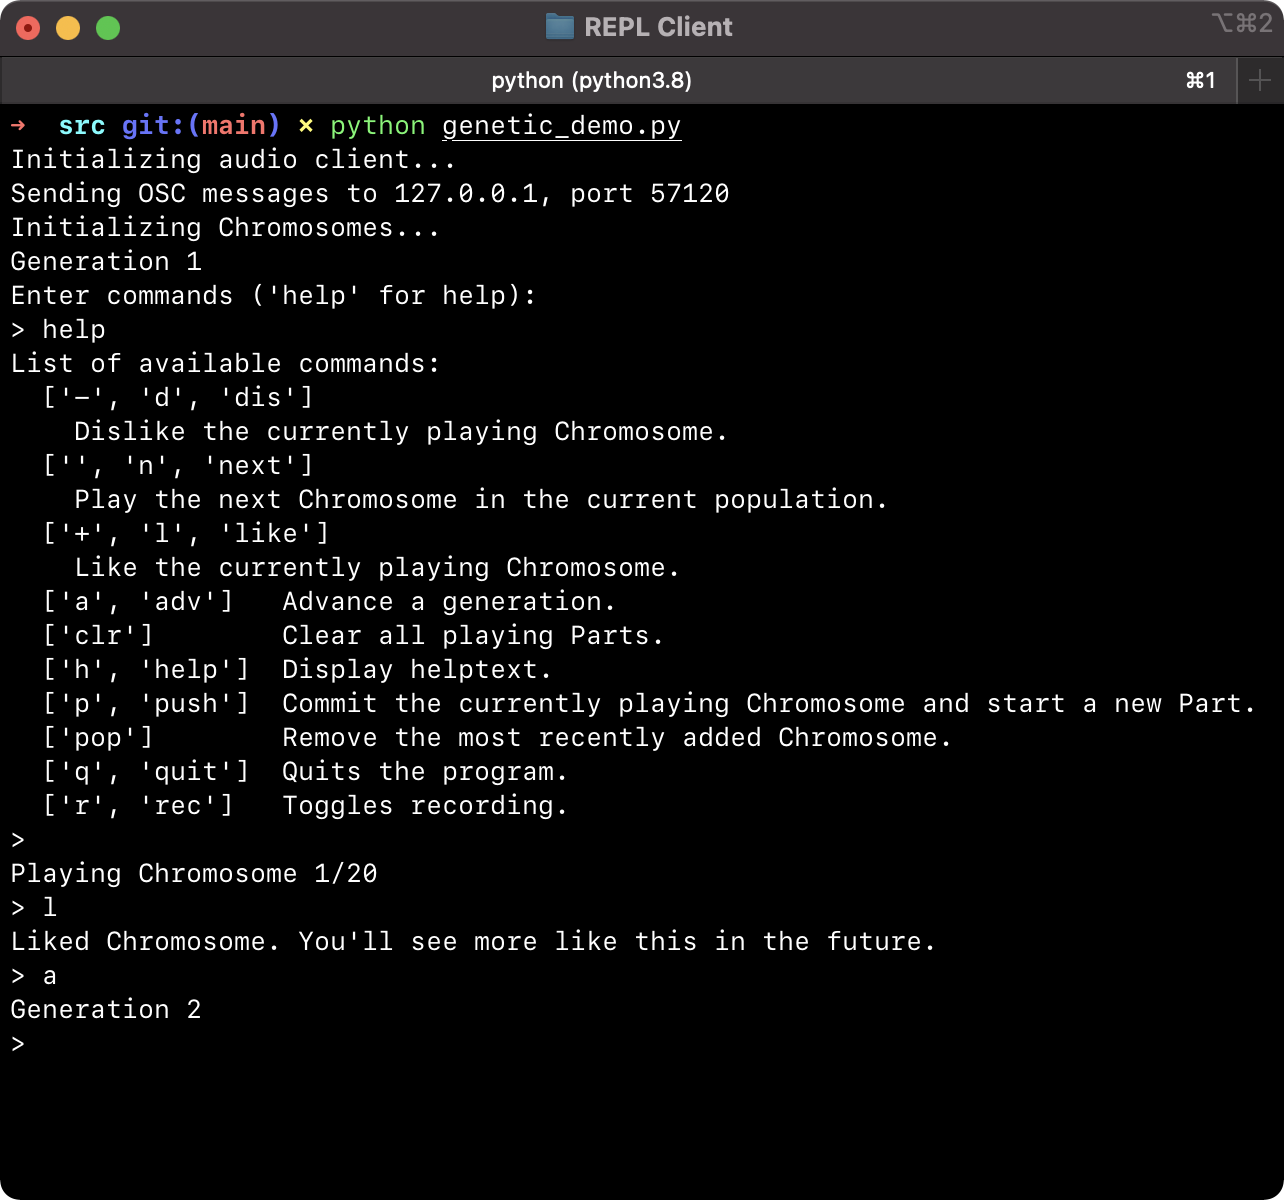
\includegraphics[width=0.9\columnwidth]{figs/repl-client.png}}
    \caption{Example run of the REPL client.}
    \label{repl}
\end{figure}

The genetic algorithm itself was developed in Python. While some Python
packages exist for performing optimization using a genetic algorithm, the
genetic algorithm here was implemented from scratch for the author's
edification. The external package scikit-learn \cite{sklearn} was used
for fitting the approximate fitness functions.

\begin{figure}[htbp]
    \centerline{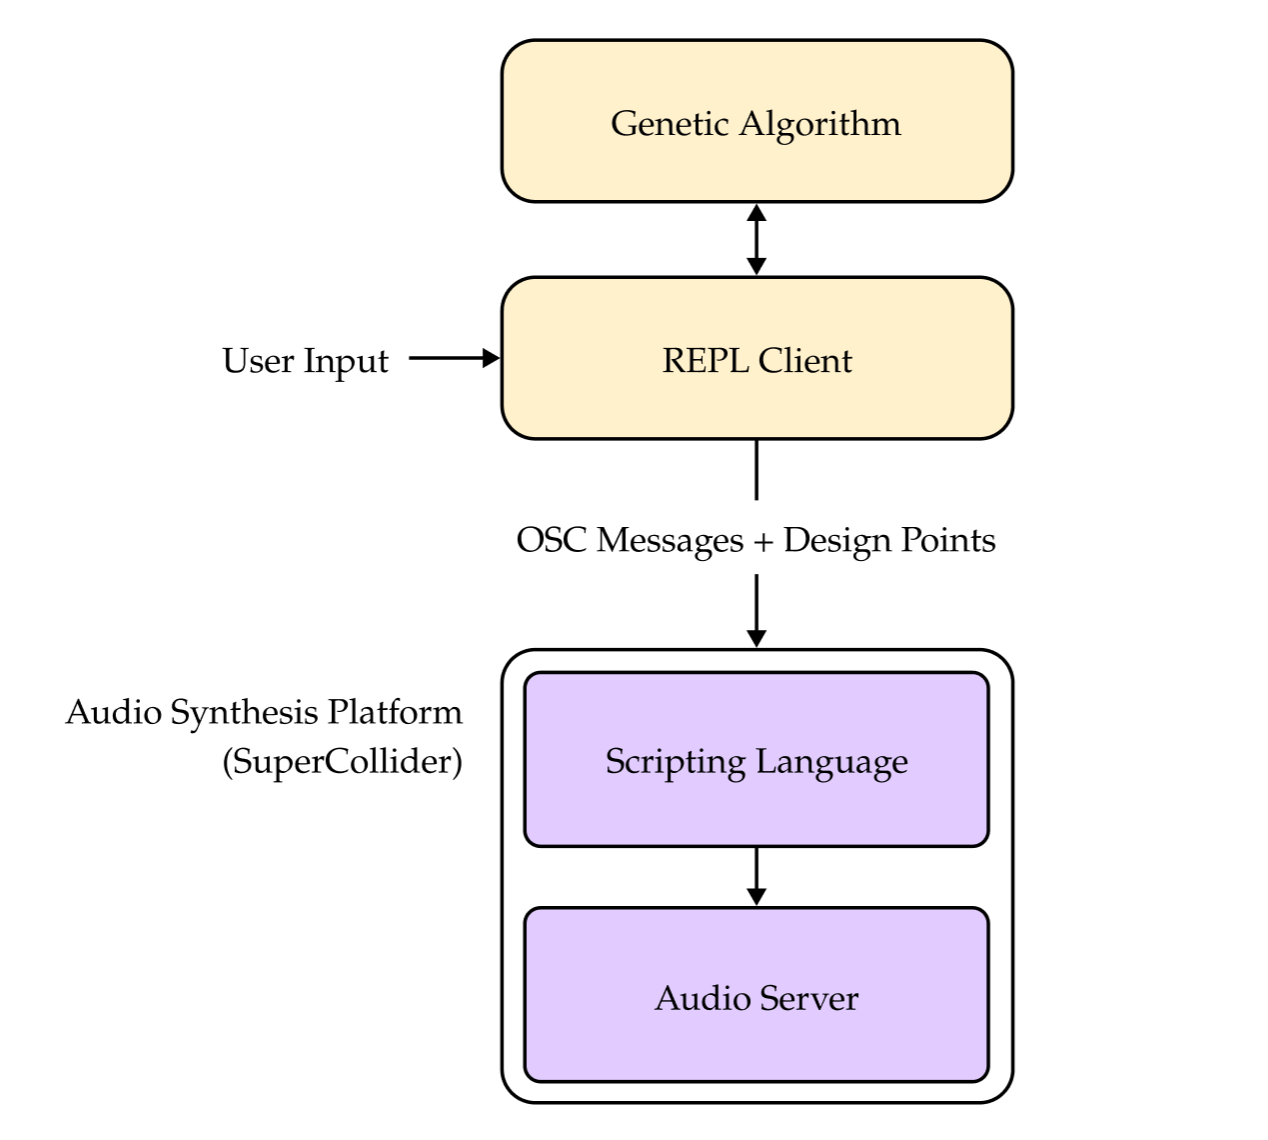
\includegraphics[width=0.9\columnwidth]{figs/arch.png}}
    \caption{Diagram capturing the interaction between the genetic
        algorithm, user input, and the sound-generating process.}
    \label{arch}
\end{figure}

\section{Results and Interpretation}

\subsection{Optimizing Test Functions}

To test the veracity and versatility of our genetic algorithm infrastructure,
we first direct the algorithm to optimize some more concrete objective
functions: Rosenbrock's and Booth's function. We alter the evolutionary
dynamics with prior knowledge of the objective function: the initial
chromosomes are points in $\mathbb{R}^2$, we use truncation selection
to more aggressively exclude less fit individuals, and we employ a mutation
strategy that frequently adds a small amount of noise to the individuals and
occasionally adds a large amount of noise.

See Fig.~\ref{test} for scatter plots of the population across
multiple generations.

\begin{figure}[htbp]
    \centering{
        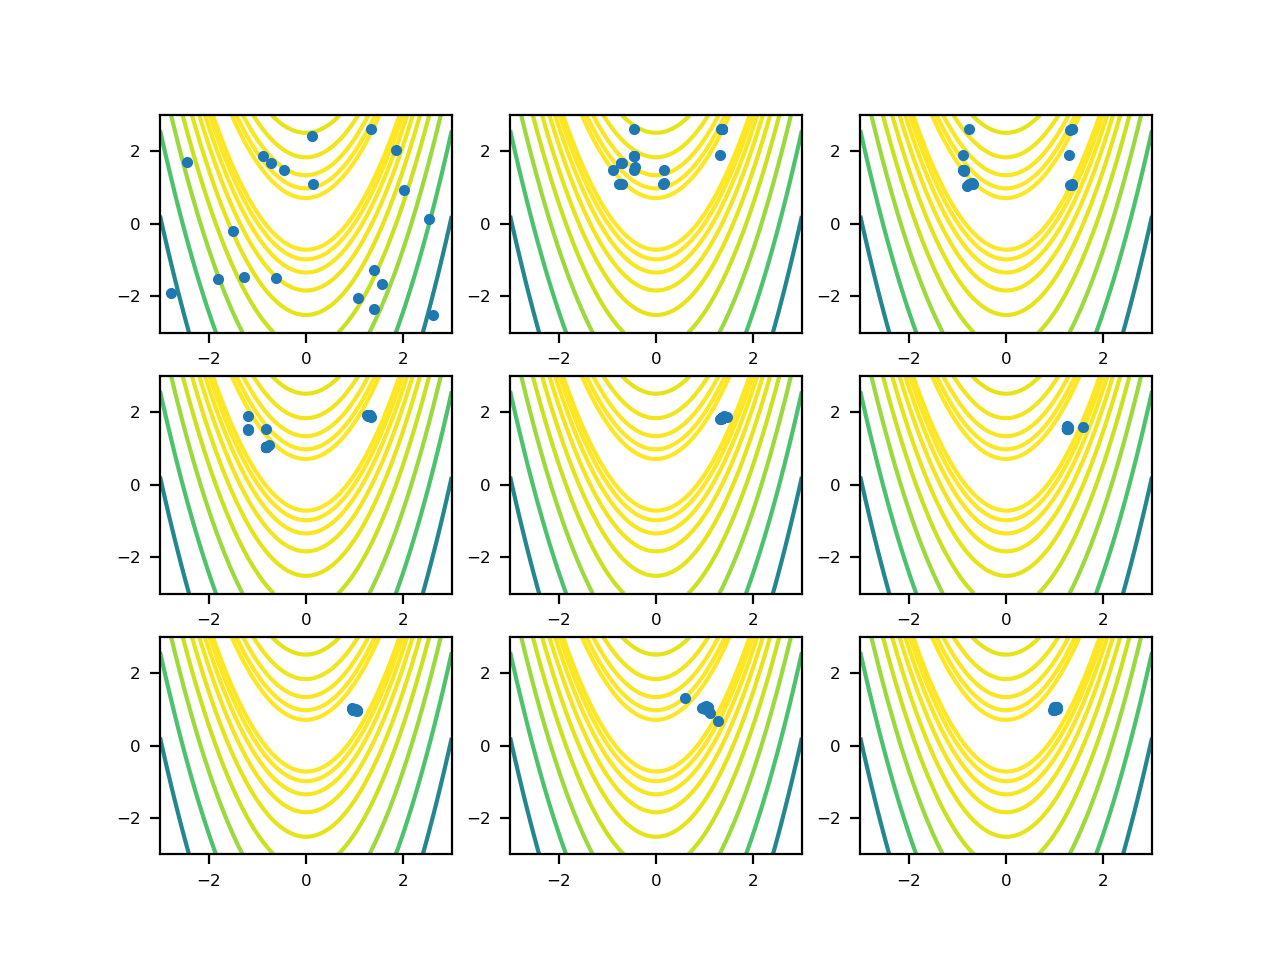
\includegraphics[width=0.99\columnwidth]{figs/rosenbrock.png}
        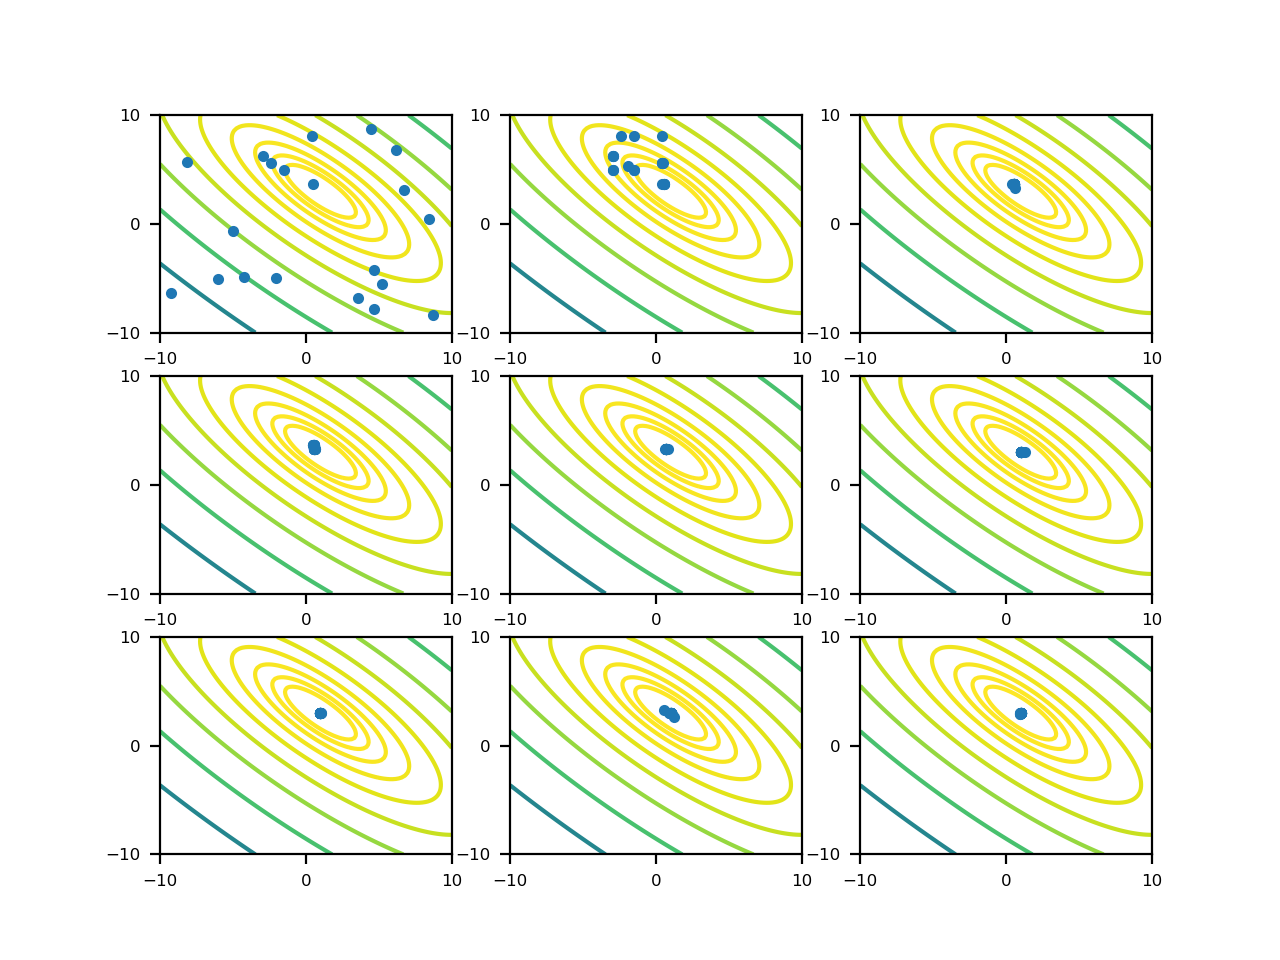
\includegraphics[width=0.99\columnwidth]{figs/booths.png}
    }
    \caption{Running genetic algorithm optimization for 999 iterations for Rosenbrock's
        function (top) and Booth's function (bottom). Plots, in reading order, are of the individuals at iteration 1 (the initial
        population), 2, 3, 5, 10, 100, 500, 900, and 1000. For reference, the global minimum of Rosenbrock's function is at $(1, 1)$.}
    \label{test}
\end{figure}

\subsection{Interpreting the User-Based Fitness Approximation}

We also interpret the efficacy and development of the fitness approximation
trained on observed user preferences. While this is a somewhat subjective thing
to evaluate, we can plot some results over the course of a run and verify the
development of the fitness approximation towards exploring points of interest.

To plot, we use t-distributed Stochastic Neighbor Embedding (t-SNE)
\cite{tsne} to project the chromosomes down to a two dimensional
representation, and we use a Voronoi tessellation \cite{hi-d-viz} to
approximate the high-dimensional decision boundary in 2D space. We make the
disclaimer that the decision boundary must lie somewhere between the positively
and negatively classified points, but in regions with few data points, the true
boundary can deviate from this. In particular, the true distances between
points, and therefore the distances between points and a decision boundary, are
warped upon projection onto a lower-dimensional space.

With a high number of dimensions, the logistic regression classifier is often
able to completely linearly separate the data (Fig.~\ref{gen1}).
We find that the next points in the design space are clustered in regions where
the user has previously liked points (Fig.~\ref{gen1} and
Fig.~\ref{gen2} ).

\begin{figure}[htbp]
    \centering{
        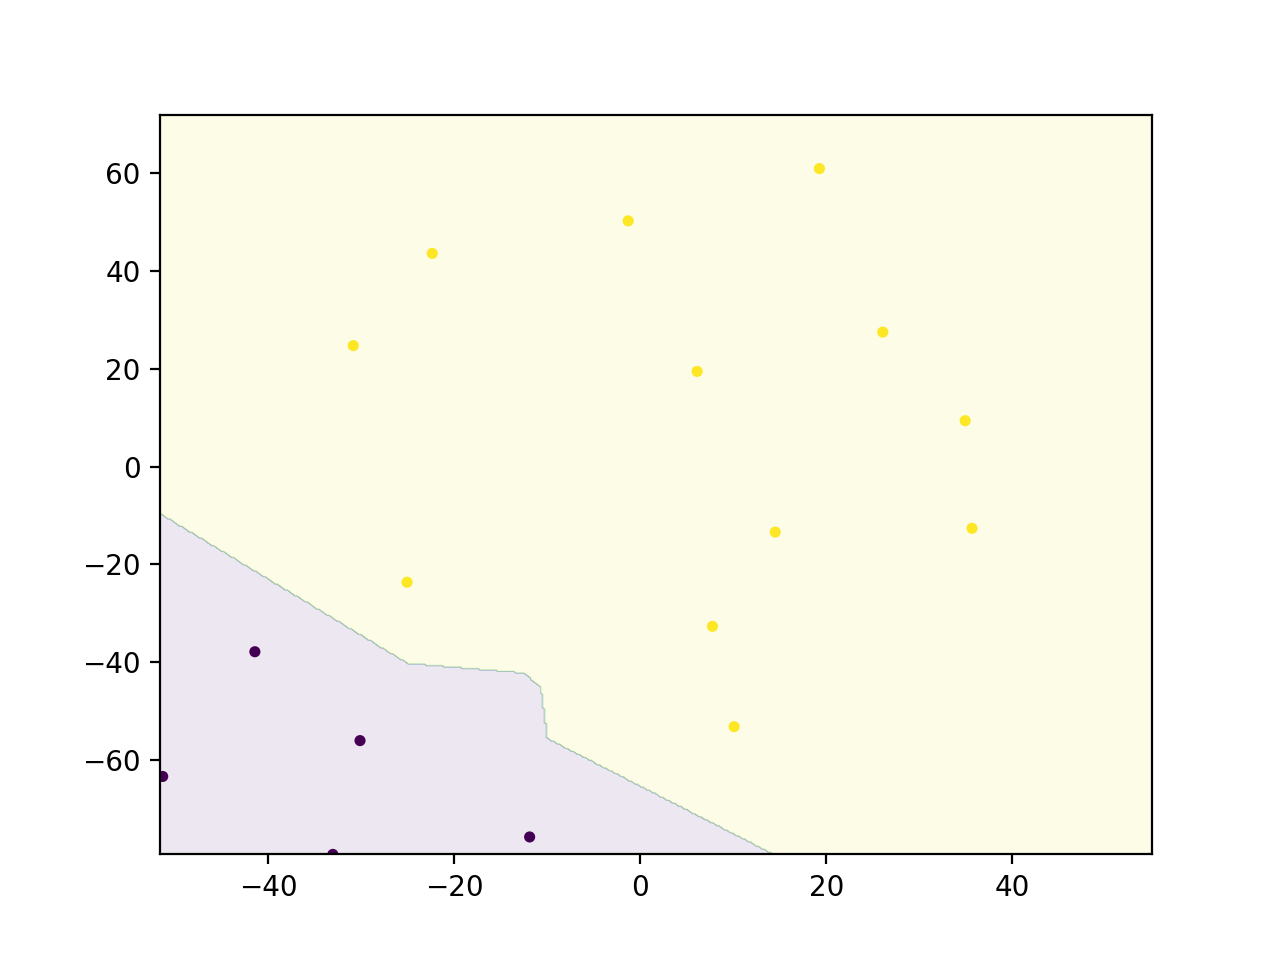
\includegraphics[width=0.45\columnwidth]{figs/dec-boundary.png}
        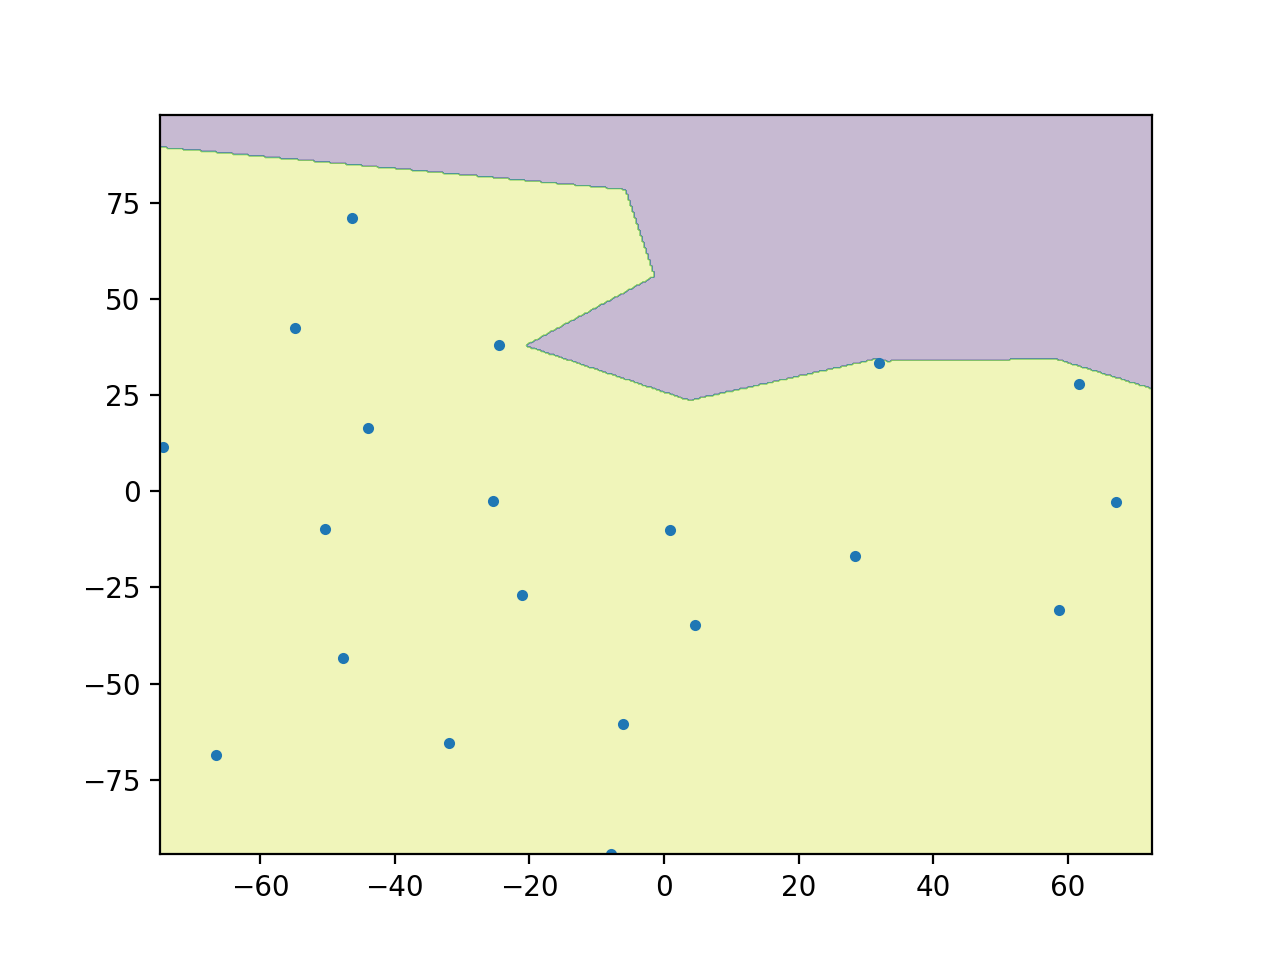
\includegraphics[width=0.45\columnwidth]{figs/new-points.png}
    }
    \caption{An example run where the surrogate model can linearly separate the data.
        Points are colored according to their true label (yellow for
        positive, purple for negative). Points in the next generation (blue) are primarily in the
        positive
        region of the
        classifier, with mutation adding some noise.}
    \label{gen1}
\end{figure}

\begin{figure}[htbp]
    \centering{
        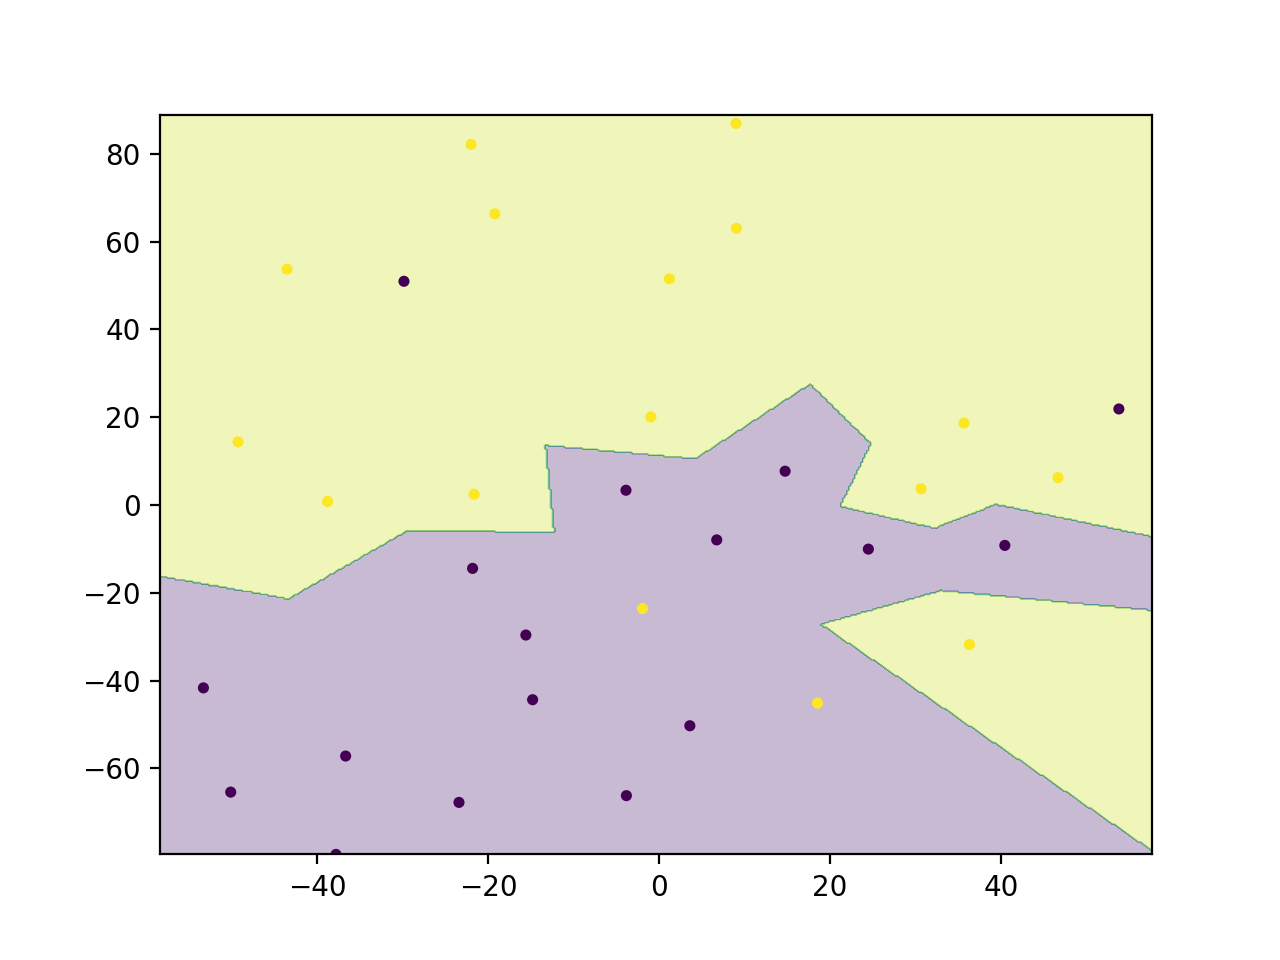
\includegraphics[width=0.45\columnwidth]{figs/dec-boundary-2.png}
        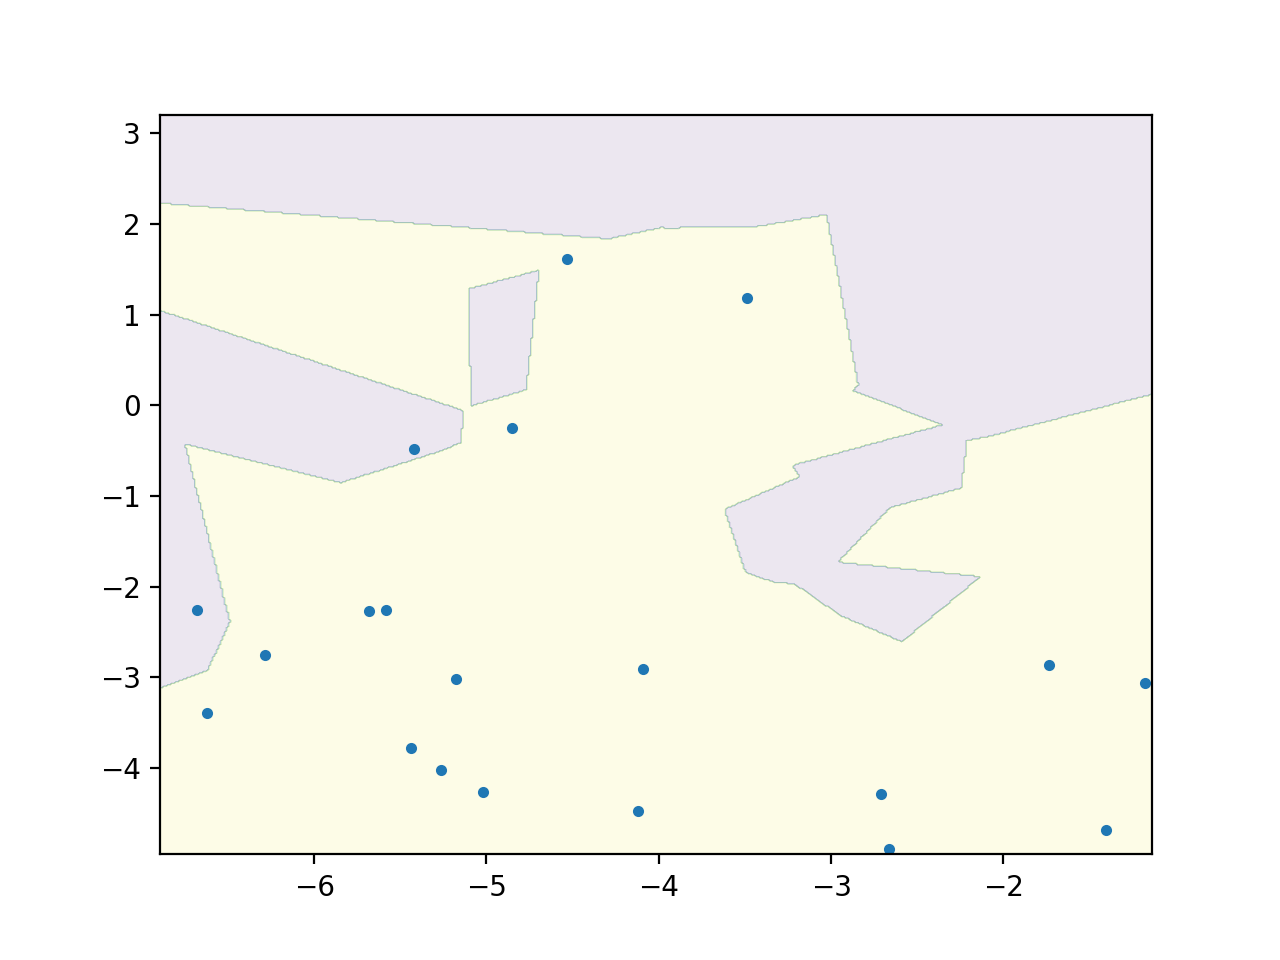
\includegraphics[width=0.45\columnwidth]{figs/new-points-2.png}
    }
    \caption{As points accumulate, the model becomes no longer able to linearly separate the data.
        Suggested points reflect the classifier's uncertainty and place some points in
        negatively classified regions.}
    \label{gen2}
\end{figure}

% We can also plot the prevalence of suggested instruments over time. Here,
% $K=6$. If the user dislikes an instrument, we should expect to
% see it less in subsequent generations.

\subsection{Generating Music}

Of course, we must make an evaluation of the music produced by the genetic
algorithm, with the usual qualifications regarding personal taste.\footnotemark
\footnotetext{The demos are hosted at \url{https://garrickf.github.io/genalg-sequencer/}, check them out!}

We find the results to be musically pleasing and rhythmically interesting,
capturing elements of the original step sequencer inspiration we sought to
reproduce. The exploration induced by the genetic algorithm allows the
discovery and experimentation with patterns and sounds one may not necessarily
find through fiddling with multiple knobs and settings on a synthesizer or
digital audio workstation (DAW). We view the genetic algorithm as an interface
to the timing and expression parameters of a synthesizer and sequencer, one
that reduces the friction for trying new things.

\section{Related Work}

Our project seeks to augment music creation through applying genetic algorithms
to the model of a synthesizer and sequencer. Horner and Goldberg also apply
genetic algorithms to music creation, focusing on the problem model of
``thematic bridging,'' which seeks to interpolate from a starting musical
pattern to a final one \cite{horner}. A solution's fitness is a
function of how closely the ending pattern matches the starting one. In
contrast, our fitness function is interactive, or dependent on user input.
Whereas the iterative process for music generation in their work involves
repeated runs of the algorithm until the results are acceptable, our work
utilizes human input to alter the fitness function of the genetic algorithm.

Matíc also applies genetic algorithms to music composition, modulating rhythms
and pitches with a predefined set of mutation operations
\cite{matic}. Similarly to Horner's and Goldberg's work, automated
criteria are used to determine the quality of a composition, related to the
evaluation of the intervals between successive notes, deviations from reference
values, and counts of implementation-defined ``bad'' tones. In contrast, our
model does not work with pitches or varied durations of notes, simplifying our
design space to that of a sequencer.

Some systems for drum loop evolution have been produced (e.g. MuSing
\cite{musing}). Our algorithm works in a similar way; however,
instead of relying on a set of fixed drum samples, we have the ability to
evolve the synthesis of sounds though the expression component of a chromosome.

Many musical artists use elements of genetic algorithms or computation in their
performance, and their tools to do so are often highly specialized. George
Lewis, one of the pioneers of computer music, created the Voyager system, which
provides live accompaniment to an instrumentalist \cite{voyager}. Al
Biles applied genetic algorithms to producing improvised jazz solos
\cite{genjazz}.

\section{Conclusion and Future Work}

In conclusion, we show an application of genetic algorithms to the creation of
music, through the lens of a sequencer/synthesizer.

More broadly, methods like these may be used for algorithmic-assisted
exploration of a large design space where function evaluations are relatively
cheap, and expert knowledge is useful. One can imagine algorithms being applied
to help designers or artists find and rapidly prototype new ideas.

It would be exciting to see an extension with more instruments and more values
and ranges for expression. For example, one such extension could add melodic
expression to the chromosome, whose coordinates encode the pitch of each note.

%%%%%%%%%%%%%%%%%% New stuff ends here.

% \section{Introduction}
% This document is a model and instructions for \LaTeX. Please observe the
% conference page limits.

% \section{Ease of Use}

% \subsection{Maintaining the Integrity of the Specifications}

% The IEEEtran class file is used to format your paper and style the text. All
% margins, column widths, line spaces, and text fonts are prescribed; please do
% not alter them. You may note peculiarities. For example, the head margin
% measures proportionately more than is customary. This measurement and others
% are deliberate, using specifications that anticipate your paper as one part of
% the entire proceedings, and not as an independent document. Please do not
% revise any of the current designations.

% \section{Prepare Your Paper Before Styling}
% Before you begin to format your paper, first write and save the content as a
% separate text file. Complete all content and organizational editing before
% formatting. Please note sections
% \ref{AA}--\ref{SCM} below for more information on
% proofreading, spelling and grammar.

% Keep your text and graphic files separate until after the text has been
% formatted and styled. Do not number text heads---{\LaTeX} will do that for you.

% \subsection{Abbreviations and Acronyms}\label{AA}
% Define abbreviations and acronyms the first time they are used in the text,
% even after they have been defined in the abstract. Abbreviations such as IEEE,
% SI, MKS, CGS, ac, dc, and rms do not have to be defined. Do not use
% abbreviations in the title or heads unless they are unavoidable.

% \subsection{Units}
% \begin{itemize}
%     \item Use either SI (MKS) or CGS as primary units. (SI units are encouraged.) English
%           units may be used as secondary units (in parentheses). An exception would be
%           the use of English units as identifiers in trade, such as ``3.5-inch disk
%           drive''.
%     \item Avoid combining SI and CGS units, such as current in amperes and magnetic field
%           in oersteds. This often leads to confusion because equations do not balance
%           dimensionally. If you must use mixed units, clearly state the units for each
%           quantity that you use in an equation.
%     \item Do not mix complete spellings and abbreviations of units:
%           ``Wb/m\textsuperscript{2}'' or ``webers per square meter'', not
%           ``webers/m\textsuperscript{2}''. Spell out units when they appear in text:
%           ``. . . a few henries'', not ``. . . a few H''.
%     \item Use a zero before decimal points: ``0.25'', not ``.25''. Use
%           ``cm\textsuperscript{3}'', not ``cc''.)
% \end{itemize}

% \subsection{Equations}
% Number equations consecutively. To make your equations more compact, you may
% use the solidus (~/~), the exp function, or appropriate exponents. Italicize
% Roman symbols for quantities and variables, but not Greek symbols. Use a long
% dash rather than a hyphen for a minus sign. Punctuate equations with commas or
% periods when they are part of a sentence, as in:
% \begin{equation}
%     a+b=\gamma\label{eq}
% \end{equation}

% Be sure that the symbols in your equation have been defined before or
% immediately following the equation. Use ``\eqref{eq}'', not
% ``Eq.~\eqref{eq}'' or ``equation \eqref{eq}'', except
% at the beginning of a sentence: ``Equation \eqref{eq} is . . .''

% \subsection{\LaTeX-Specific Advice}

% Please use ``soft'' (e.g., \verb|\eqref{Eq}|) cross references instead of
% ``hard'' references (e.g., \verb|(1)|). That will make it possible
% to combine sections, add equations, or change the order of figures or citations
% without having to go through the file line by line.

% Please don't use the \verb|{eqnarray}| equation environment. Use
% \verb|{align}| or \verb|{IEEEeqnarray}| instead. The
% \verb|{eqnarray}|
% environment leaves unsightly spaces around relation symbols.

% Please note that the \verb|{subequations}| environment
% in {\LaTeX} will increment the main equation counter even
% when there are no equation numbers displayed. If you forget that, you might
% write an article in which the equation numbers skip from (17) to (20), causing
% the copy editors to wonder if you've discovered a new method of
% counting.

%     {\BibTeX} does not work by magic. It doesn't get the
% bibliographic data from thin air but from .bib files. If you
% use {\BibTeX} to produce a bibliography you must send the .bib
% files.

%     {\LaTeX} can't read your mind. If you assign the same
% label to a subsubsection and a table, you might find that Table I has been
% cross referenced as Table IV-B3.

% {\LaTeX} does not have precognitive abilities. If you put a
% \verb|\label| command before the command that updates the counter it's
% supposed to be using, the label will pick up the last counter to be cross
% referenced instead. In particular, a \verb|\label| command should not
% go before the caption of a figure or a table.

% Do not use \verb|\nonumber| inside the \verb|{array}|
% environment. It will not stop equation numbers inside \verb|{array}|
% (there won't be any anyway) and it might stop a wanted equation number in the
% surrounding equation.

% \subsection{Some Common Mistakes}\label{SCM}
% \begin{itemize}
%     \item The word ``data'' is plural, not singular.
%     \item The subscript for the permeability of vacuum $\mu_{0}$, and other
%           common scientific constants, is zero with subscript formatting, not a lowercase
%           letter ``o''.
%     \item In American English, commas, semicolons, periods, question and exclamation
%           marks are located within quotation marks only when a complete thought or name
%           is cited, such as a title or full quotation. When quotation marks are used,
%           instead of a bold or italic typeface, to highlight a word or phrase,
%           punctuation should appear outside of the quotation marks. A parenthetical
%           phrase or statement at the end of a sentence is punctuated outside of the
%           closing parenthesis (like this). (A parenthetical sentence is punctuated within
%           the parentheses.)
%     \item A graph within a graph is an ``inset'', not an ``insert''. The word
%           alternatively is preferred to the word ``alternately'' (unless you really mean
%           something that alternates).
%     \item Do not use the word ``essentially'' to mean ``approximately'' or
%           ``effectively''.
%     \item In your paper title, if the words ``that uses'' can accurately replace the word
%           ``using'', capitalize the ``u''; if not, keep using lower-cased.
%     \item Be aware of the different meanings of the homophones ``affect'' and ``effect'',
%           ``complement'' and ``compliment'', ``discreet'' and ``discrete'', ``principal''
%           and ``principle''.
%     \item Do not confuse ``imply'' and ``infer''.
%     \item The prefix ``non'' is not a word; it should be joined to the word it modifies,
%           usually without a hyphen.
%     \item There is no period after the ``et'' in the Latin abbreviation ``et al.''.
%     \item The abbreviation ``i.e.'' means ``that is'', and the abbreviation ``e.g.''
%           means ``for example''.
% \end{itemize}
% An excellent style manual for science writers is \cite{b7}.

% \subsection{Authors and Affiliations}
% \textbf{The class file is designed for, but not limited to, six authors.} A
% minimum of one author is required for all conference articles. Author names
% should be listed starting from left to right and then moving down to the next
% line. This is the author sequence that will be used in future citations and by
% indexing services. Names should not be listed in columns nor group by
% affiliation. Please keep your affiliations as succinct as possible (for
% example, do not differentiate among departments of the same organization).

% \subsection{Identify the Headings}
% Headings, or heads, are organizational devices that guide the reader through
% your paper. There are two types: component heads and text heads.

% Component heads identify the different components of your paper and are not
% topically subordinate to each other. Examples include Acknowledgments and
% References and, for these, the correct style to use is ``Heading 5''. Use
% ``figure caption'' for your Figure captions, and ``table head'' for your table
% title. Run-in heads, such as ``Abstract'', will require you to apply a style
% (in this case, italic) in addition to the style provided by the drop down menu
% to differentiate the head from the text.

% Text heads organize the topics on a relational, hierarchical basis. For
% example, the paper title is the primary text head because all subsequent
% material relates and elaborates on this one topic. If there are two or more
% sub-topics, the next level head (uppercase Roman numerals) should be used and,
% conversely, if there are not at least two sub-topics, then no subheads should
% be introduced.

% \subsection{Figures and Tables}
% \paragraph{Positioning Figures and Tables} Place figures and tables at the top and
% bottom of columns. Avoid placing them in the middle of columns. Large figures
% and tables may span across both columns. Figure captions should be below the
% figures; table heads should appear above the tables. Insert figures and tables
% after they are cited in the text. Use the abbreviation
% ``Fig.~\ref{fig}'', even at the beginning of a sentence.

% \begin{table}[htbp]
%     \caption{Table Type Styles}
%     \begin{center}
%         \begin{tabular}{|c|c|c|c|}
%             \hline
%             \textbf{Table} & \multicolumn{3}{|c|}{\textbf{Table Column Head}}                                                         \\
%             \cline{2-4}
%             \textbf{Head}  & \textbf{\textit{Table column subhead}}           & \textbf{\textit{Subhead}} & \textbf{\textit{Subhead}} \\
%             \hline
%             copy           & More table copy$^{\mathrm{a}}$                   &                           &                           \\
%             \hline
%             \multicolumn{4}{l}{$^{\mathrm{a}}$Sample of a Table footnote.}
%         \end{tabular}
%         \label{tab1}
%     \end{center}
% \end{table}

% \begin{figure}[htbp]
%     \centerline{
\includegraphics{fig1.png}}
%     \caption{Example of a figure caption.}
%     \label{fig}
% \end{figure}

% Figure Labels: Use 8 point Times New Roman for Figure labels. Use words rather
% than symbols or abbreviations when writing Figure axis labels to avoid
% confusing the reader. As an example, write the quantity ``Magnetization'', or
% ``Magnetization, M'', not just ``M''. If including units in the label, present
% them within parentheses. Do not label axes only with units. In the example,
% write ``Magnetization (A/m)'' or ``Magnetization
% \{A[m(1)]\}'', not just ``A/m''. Do not label axes with a
% ratio of quantities and units. For example, write ``Temperature (K)'', not
% ``Temperature/K''.

% \section*{Acknowledgment}

% The preferred spelling of the word ``acknowledgment'' in America is without an
% ``e'' after the ``g''. Avoid the stilted expression ``one of us (R. B. G.)
% thanks $\ldots$''. Instead, try ``R. B. G.
% thanks$\ldots$''. Put sponsor acknowledgments in the unnumbered
% footnote on the first page.

% \section*{References}

% Please number citations consecutively within brackets \cite{b1}.
% The sentence punctuation follows the bracket \cite{b2}. Refer
% simply to the reference number, as in \cite{b3}---do not use
% ``Ref. \cite{b3}'' or ``reference \cite{b3}''
% except at the beginning of a sentence: ``Reference \cite{b3} was
% the first $\ldots$''

% Number footnotes separately in superscripts. Place the actual footnote at the
% bottom of the column in which it was cited. Do not put footnotes in the
% abstract or reference list. Use letters for table footnotes.

% Unless there are six authors or more give all authors' names; do not use ``et
% al.''. Papers that have not been published, even if they have been submitted
% for publication, should be cited as ``unpublished'' \cite{b4}.
% Papers that have been accepted for publication should be cited as ``in press''
% \cite{b5}. Capitalize only the first word in a paper title,
% except for proper nouns and element symbols.

% For papers published in translation journals, please give the English citation
% first, followed by the original foreign-language citation
% \cite{b6}.

\begin{thebibliography}{00}
    % \bibitem{b1} G. Eason, B. Noble, and I. N.
    % Sneddon, ``On certain integrals of Lipschitz-Hankel type involving products of
    % Bessel functions,'' Phil. Trans. Roy. Soc. London, vol. A247, pp. 529--551,
    % April 1955. \bibitem{b2} J. Clerk Maxwell, A Treatise on Electricity
    % and Magnetism, 3rd ed., vol. 2. Oxford: Clarendon, 1892, pp.68--73.
    % \bibitem{b3} I. S. Jacobs and C. P. Bean, ``Fine particles, thin
    % films and exchange anisotropy,'' in Magnetism, vol. III, G. T. Rado and H.
    % Suhl, Eds. New York: Academic, 1963, pp. 271--350. \bibitem{b4} K.
    % Elissa, ``Title of paper if known,'' unpublished. \bibitem{b5} R.
    % Nicole, ``Title of paper with only first word capitalized,'' J. Name Stand.
    % Abbrev., in press. \bibitem{b6} Y. Yorozu, M. Hirano, K. Oka, and Y.
    % Tagawa, ``Electron spectroscopy studies on magneto-optical media and plastic
    % substrate interface,'' IEEE Transl. J. Magn. Japan, vol. 2, pp. 740--741,
    % August 1987 [Digests 9th Annual Conf. Magnetics Japan, p. 301, 1982]. \bibitem{b7} M. Young, The
    % Technical Writer's Handbook. Mill Valley, CA: University Science, 1989.

    % Problem
    \bibitem{sequencers} ``Music sequencer," \url{https://en.wikipedia.org/wiki/Music_sequencer} (accessed May 2021).

    % Method
    \bibitem{genalg-textbook} D.E. Goldberg, \textit{Genetic Algorithms in Search, Optimization, and Machine Learning}, Addison-Wesley,
    1989.

    \bibitem{textbook} M.J. Kochenderfer and T.A. Wheeler,
    \textit{Algorithms for Optimization}, MIT Press, 2018.

    % Implementation
    \bibitem{sc} ``Supercollider: supercollider,"
    \url{https://supercollider.github.io/} (accessed May 2021).

    \bibitem{osc} M. Wright and A. Freed, "Open sound control: a new
    protocol for communicating with sound synthesizers," in International Computer
    Music Conference (ICMC), 1997, pp. 101-104. \bibitem{sklearn}
    "Scikit-learn: machine learning in python," \url{https://scikit-learn.org/stable/} (accessed May 2021).

    % Results
    \bibitem{tsne} L.J.P. van der Maaten and G.E. Hinton, ``Visualizing
    high-dimensional data using t-sne," in Journal of Machine Learning Research
    vol. 9, 2008, pp. 2579-2605.

    \bibitem{hi-d-viz} M.A. Migut, M. Worring, and C.J. Veenman, ``Visualizing
    multi-dimensional decision boundaries in 2d," in Data Mining and Knowledge
    Discovery, vol. 29, 2015, pp. 273-295.

    % Related Work
    \bibitem{horner} A. Horner and D. E. Goldberg, ``Genetic algorithms and
    computer-assisted music composition," January 1991.

    \bibitem{matic} D. Matíc, ``A genetic algorithm for composing music,"
    Yugoslav Journal of Operations Research, vol. 20, pp. 157-177, April 2010.

    \bibitem{musing} ``MuSing,'' \url{http://www.geneffects.com/musing/} (accessed
    May 2021).

    \bibitem{voyager} G.E. Lewis, ``Too many notes: computers, complexity and
    culture in voyager," Leonardo Music Journal, vol. 10, pp. 33-39, 2000.

    \bibitem{genjazz} J.A. Biles, ``GenJam: a genetic algorithm for generating
    jazz solos," International Computer Music Conference, pp. 131-137, July 1994.

\end{thebibliography}
% \vspace{12pt}
% \color{red}
% IEEE conference templates contain guidance text for composing and formatting
% conference papers. Please ensure that all template text is removed from your
% conference paper prior to submission to the conference. Failure to remove the
% template text from your paper may result in your paper not being published.

\end{document}
